\section{Image processing}

Support for visual processing is a mandatory requirement for a
software library designed to be used in humanoid robotics. Real time
systems are critical for vision, as computer vision algorithms require
the elaboration of a large quantity of data.

Efficiency is very important in image processing, so we choose
an approach which interfaces particularly well with popular
optimized libraries, but which is still capable of good
performance in their absence.

To help developers write efficient visual processing routines, Intel
released the Image Processing Library (IPL). This library in optimized
to provide high performance on machines which employ Intel processors,
especially if equipped with MMX\texttrademark technology. The IPL
library is a set of C functions which implement basic operations on
images, from simple algebraic operations on pixels to color
conversions and convolutions. The library consists of different
modules optimized for different CPU. For better performance at
run-time the library automatically detects the CPU type and loads the
module that is more suitable. Another advantage of using the IPL is
that it is at the core of the OpenCV library
(http://sourceforge.net/projects/opencvlibrary/) which provides 
sophisticated routines for image processing such as filtering, face
tracking, optic flow, and much more.

Our basic image class (YARPImage) has an internal structure that is
compatible with the IPL library.  This allows any user to take full
advantage of the IPL and/or OpenCV libraries; if these libraries
are not used, then a core set of functions are available through
YARP.  Furthermore, the image class can act as a {\em proxy} to image
data stored in a foreign format.  This is useful to prevent unnecessary
copies when using other image processing libraries, or interfacing
with image sources (e.g. framegrabbers) and sinks (e.g. a graphic
display).


%% Unfortunately the IPL library does not provide support for object
%% oriented programming. We decided to write a library which implements a
%% set of classes to store and manipulate the pixels of an image. The set
%% of classes is in the form of a C++ template that can be instantiated
%% for each pixel type (for example at the moment RGB, grayscale and
%% floating point are implemented). The YARPImageOf template defines an
%% interface for all the image classes in the library; as in other parts
%% of the library we decided to use templates for efficiency reasons. The
%% internal structure of the image is identical to the one used by the
%% IPL library. 


YARP also provides support for transmitting images between two YARP
ports.


\begin{figure}[t]
\centerline{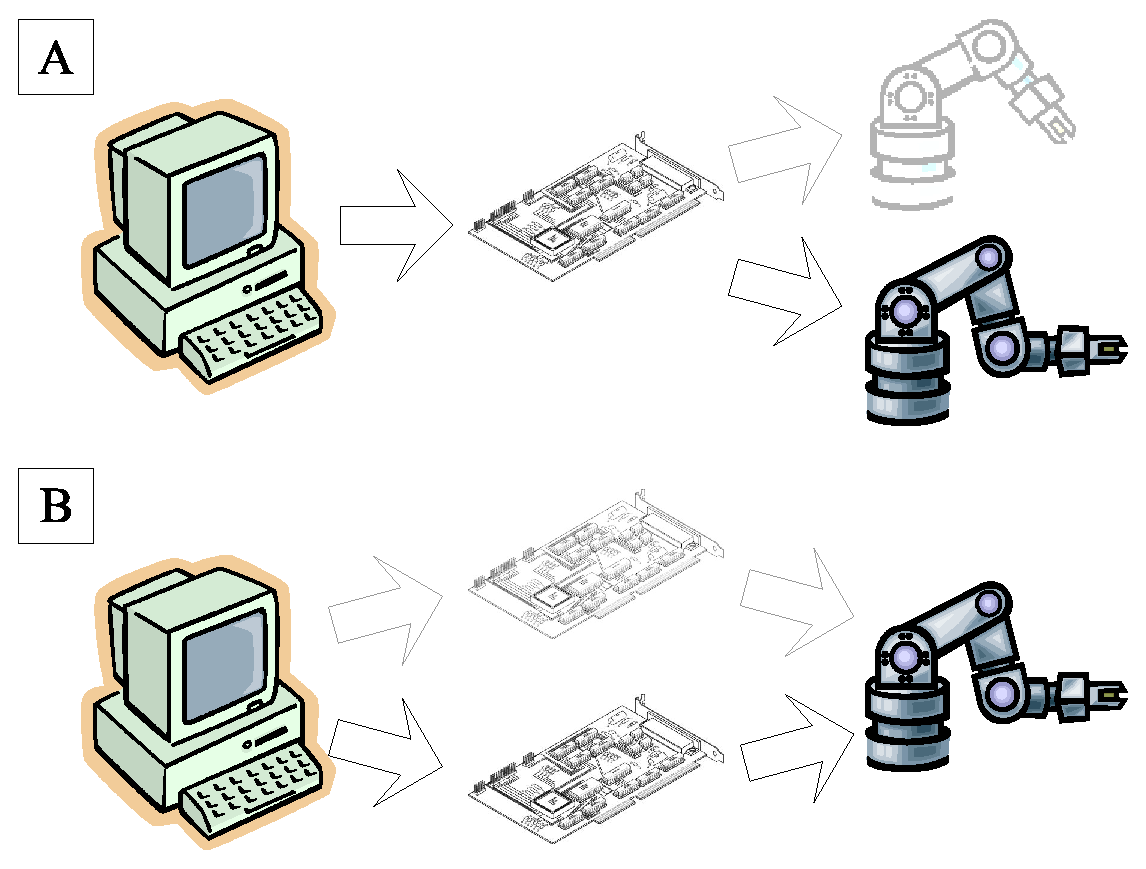
\includegraphics[width=\columnwidth]{fig-devices}}
\caption{
devices
}
\end{figure}

\section{Device drivers}

A frequent problem encountered during development in robotics is that
it is very hard to reuse code on different platforms. In some cases
this cannot be avoided, especially when the platforms are mechanically
different. In other cases, however the platforms are mechanically
similar, or just mount different boards. For example this happens when
two robots have different frame grabbers, or different control
boards. In these situations it is not possible to reuse code written
for a platform on the other. However something can be done to reduce
the differences and localize them to specific components. The idea is
that high level software modules are not (or should not be) concerned
with the low level details of the underlying hardware platform.

We defined a virtual device driver interface into YARP and
encapsulated the control parts of the robot into a standardized
template class hierarchy. The structure of the YARP virtual device
driver resembles the structure of UNIX device drivers. It has three
main methods: Open, Close and Ioctl. Open and Close execute code to
initialize and quit the device, whereas the IOCtl is the core of the
interface and consists in a set of messages. Each message defines an
index in a table of functions. The advantage of using this structure
as opposed to a virtual class is that it is not mandatory to implement
all methods if some are not supported by the hardware.

The low level software should capture the essential functioning of the
particular class of device and hide the details of the
implementation. For example the device driver for a control board
should provide methods for moving a joint by specifying the desired
position, velocity and acceleration. Other common functionalities are
methods to read position, speed and torque (if available). In practice
the main differences between cards lay on the steps required for the
initialization of the device. This approach has been successfull with
general purpose hardware like frame grabbers and control boards but
might fail to scale to custom devices like dedicated DSP for motion
control. In these cases it is harder (if not impossible) to identify a
common interface and it is best to provide a separate set of functions
to handle the specific functionalities of each device.

[this can be a good point to cut the text if the following part is too abscure or the paper is too long]

A somewhat opposite problem occurs when two identical boards are used
on setups that are mechanically different. Experience shows that in
these situations code reuse is very difficult. Consider for instance
the example of two robotic arms controlled by identical boards. The
calibration of the joints might be different if indexes are available
in the encoders or if hardware limits are presents in the
joints. Likewise, the procedure required to activate the amplifiers
might differ in the two cases. These dissimilarities cannot be handled
by different configuration files as they imply the execution of
different routines.

The ensemble of these routines are grouped in the adapter. This class
is in general responsible of implementing methods to correctly
initialize and quit the device, but it can implement other
functionalities as well. The adapter is hence the place where all the
peculiarities of each piece of hardware (and of the device used to
interface to it) are handled. As such it collects all and the only
routines specific to each hardware device.

Finally, device driver and adapter are aggregated together by a single
class. The interface between higher level software modules and the
hardware occurs through this class and is thus independent of the
device driver or the actual hardware underneath. Code changes required
to use different boards or mechanical devices are localized to the
device driver and the adapter respectively.

\subsection{Device Driver Example: YARPGenericFrameGrabber}

As an exemple we report here the structure of the generic frame grabber. The first layer is the YARPDeviceDriver which defines the methods open(), close() and IOCtl(). It also stores the function table that implements the interface of the drivere (m\_cmds); this table is allocated and initialized in the YARPDeviceDriver constructor. This table is correcly filled by the DERIVED class (see below).

{\small \begin{verbatim}
template <class DERIVED>
class YARPDeviceDriver
{
public:
	YARPDeviceDriver(int n_cmds);
	virtual ~YARPDeviceDriver();
protected:
	typedef int (DERIVED::*cmd_function_t)(void *);
	// function table
	cmd_function_t *m_cmds;

public:
	virtual int open(void *p) = 0;
	virtual int close() = 0;

	int IOCtl(int cmd, void *data)
	{
	  int ret = ((DERIVED *)
	            this->*m_cmds[cmd])(data);
	  return ret;
	}
};
\end{verbatim} }

In addition we defined the following messages:

{\small \begin{verbatim}
enum FrameGrabberCmd
{
  FCMDWaitNewFrame,
  FCMDAcquireBuffer,
  FCMDReleaseBuffer,
  FCMDGetSizeX,
  FCMDGetSizeY,
  FCMDSetContrast,
  ...
};
\end{verbatim} }

The first message waits for a new frame to be acquired. FCMDAcquireBuffer reserves the most recent frame and returns a pointer to it; the frame is released by the application by calling FCMDReleaseBuffer. The other messages are simple commands to set/get general parameters.

The YARPGenericGrabberAdapter is a virtual class which defines the interface for the adapter. In this case it is quite simple and consists only in the initialize() and uninitialize() methods. 

The last layer is a template class YARPGenericGrabber whose parameter is the adapter of a specific board. Part of the implementation of the YARPGenericGrabber is reported here:

{\small \begin{verbatim}
template <class ADAPTER>
class YARPGenericGrabber
{
protected:
	ADAPTER _adapter;
public:
	YARPGenericGrabber ();
	~YARPGenericGrabber ();

	int initialize (...)
	{
	  return  _adapter.initialize(...);
	}

	int uninitialize ()
	{
	  return _adapter.uninitialize();
	}

	int acquireBuffer (unsigned char **buffer)
	{
	  return _adapter.IOCtl(FCDMAcquireBuffer, 
	                        buffer);
	}

	int releaseBuffer (void)
	{
	  return _adapter.IOCtl(FCMDReleaseBuffer);
	}

	int setContrast(unsigned int contrast)
	{
	  return _adapter.IOCtl(FCMDSetContrast, 
	                        &contrast);
	}

	... //other methods
}
\end{verbatim} }

To instantiate and use the YARPGenericGrabber in our code we need to define the classes implementing the device driver and the adapter for the particular board we intend to use (respectively MyDeviceDriver and MyGrabberAdapter). MyDeviceDriver derives from YARPDeviceDriver. It implements open() and close() methods. The frame grabber interface is implemented in the form of a set of functions whose pointers are stored in m\_cmds. MyDeviceDriver does not need to implement all messages but only the subset of the ones that are meaningful for the board actually in use. This is perfectly safe because by default each entry of the table is initialized to point to an empty (but valid) function.

{\small \begin{verbatim}
class MyDeviceDriver : 
	public YARPDeviceDriver<MyDeviceDriver>
{
  MyDeviceDriver()
  {
    // fils function table
    m_cmds[FCMDAcquireBuffer] =
                     &MyDeviceDriver::acquireBuffer;
    m_cmds[FCMDReleaseBuffer] =
                     &MyDeviceDriver::releaseBuffer;
    m_cmds[FCMDFaitFrame] = 
                     &MyDeviceDriver::waitOnFrame;
    ...
  }

  // open and initialize the device
  int open(void *d);

  // close the device
  int close(void);

protected:
  // messages:
  int waitOnFrame(void *cmd);
  int acquireBuffer(void *buffer);
  int releaseBuffer(void *cmd);
  ...
}
\end{verbatim}}

 The MyGrabberAdapter implements only and all the methods defined in the YARPGenericGrabberAdapter. It also derives from MyGenericDeviceDriver to allow accessing the device driver from the higher level layer. A possible implementation is reported here:

{\small \begin{verbatim}
class MyGrabberAdapter: 
	public MyDeviceDriver,
	public YARPGenericGrabberAdapter
{
  int initialize(...)
  {
    MyDeviceDriver::open();
    MyDeviceDriver::IOCtl(FCMSetContrast, ...);
    ... // other initializations
    return YARP_OK;
  }

  int unitialize()
  {
    MyDeviceDriver::close();
    ...
  }
}
\end{verbatim}}

Having implemented the adapter and the device driver for our frame grabber, it is now sufficient to instantiate and use the YARPGenericGrabber as follows:

{\small
\begin{verbatim}

typedef YARPGenericGrabber<MyGrabberAdapter> 
                          YARPGrabber;

int main()
{
  YARPGrabber _grabber;
  // initialize device
  _grabber.initialize(..);
  
  bool done = false;

  while(!done)
  {
    // wait until a new frame is ready
    _grabber.waitOnNewFrame();
    // lock most recent frame and
    // get a pointer to it
    _grabber.acquireBuffer(&buffer);
    // ...
    // ...
    // release frame
    _grabber.releaseBuffer();
  }

  // close the device
  _grabber.uninitialize();
}
\end{verbatim}
}